\documentclass[a4paper]{article}

\usepackage[T1]{fontenc}
\usepackage[adobe-utopia]{mathdesign}
\usepackage[protrusion=true,expansion=true]{microtype}
\usepackage{xcolor}
\usepackage{graphicx}

\definecolor{darkblue}{rgb}{0,0,0.5}

\usepackage[colorlinks=true,
        urlcolor=darkblue,
        anchorcolor=darkblue,
        linkcolor=darkblue,
        citecolor=darkblue,
        pdfauthor={Mohannad Banayosi},
        pdfkeywords={educational tools, pseudo-code, virtual machine,
          parser, interpreter},
        pdftitle={Real-time fitness monitor.},
        pdfsubject={Real-time fitness monitor,
          the German University in Cairo GUC
          (http://met.guc.edu.eg/)}]{hyperref}
\usepackage{url}

\author{Mohannad Banayosi}
\title{Real-time fitness monitor.}

\begin{document}

\maketitle

\begin{abstract}
IMPACT is a multidisciplinary project in which students of computer science (more precisely: software engineering), material sciences, mechatronics and embedded system design come together to create Thai-boxing pads with builtin impact sensors and wireless connection to a base station.
In this project, we will implement a multi-sensor tracking and analysis tool for a physical workout routine specific to Thai/kick-boxing or similar contact sports to track and display performance and fitness level of a practitioner over a single and over multiple sessions. It will be used to record and correlate the inputs from impact sensors and technique recognition and track improvemets of practitioners over time.
  
\end{abstract}

\newpage

\section{Background}
\begin{figure}[h!]
\centering
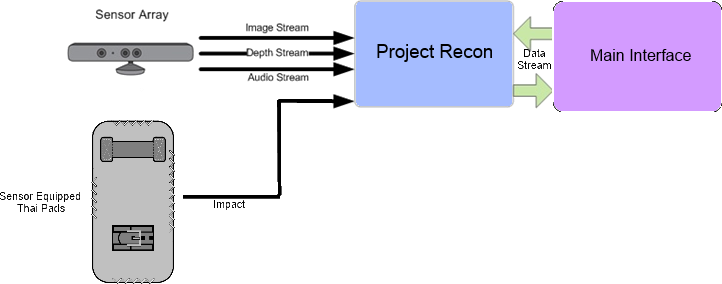
\includegraphics[scale=0.6]{General.png}
\caption{General Overview}
\label{threadsVsSync}
\end{figure}

\subsection{Problem}
In the world of martial arts, there is no accurate way to study and analyze the performance of the trainee. This absence of analysis is due to the lack of tools presented to the trainers.

\subsection{Aim of this project}
The aim of this project is to deliver an easy-to-use interface that displays training sessions' info and statistics. This in turn will help the trainers to get an accurate analysis of the trainee's performance.

\subsection{Technologies and frameworks researched}
A lot of technologies and frameworks have been researched, some of them were chosen to be used and others not. Following is a list of them.
Most of the technologies researched where not used because of their violation of the core feature of the interface being generic.

\subsubsection{Depthjs}
Depthjs was developed by four MIT students, Aaron Zinman, Doug Fritz, Greg Elliott and Roy Shilkrot in 2010. Depthjs allows any web page to interact with the Microsoft Kinect using Javascript. It provides the low-level raw access to the Kinect as well as high-level hand gesture events to simplify development.
\\* Depthjs is an open source project, but with no enough documentation, compatible with Google chrome only, and is more helpful in web navigation.

\newpage

\subsubsection{Zigfu}
Zigfu was developed by Ted Blackman, Shlomo Zippel, Roee Shenberg, Amir Hirsch, Bryce Tucker. They developed the ZDK (Zigfu Development Kit) to make cross-platform, motion-controlled apps with Kinect in HTML5/Javascript, Unity3D and Flash. Applications made with this development kit are portable across all operating systems, web browsers, computer vision middlewares, and 3D sensors. 
\\*Zigfu is not an open source project, still have problems in performance and accuracy in gesture recognition.


\subsubsection{OpenDepth}
OpenDepth - Extending the Web - is a client server application developed by Ecaterina Paun, Narcis Paun and Mircea Piturca. OpenDepth brings Kinect SDK methods and data to the web with the server side written on C\# and built on top of Kinect SDK 1.5, while the client side is a written in JavaScript and uses the Three.js webGL rendering engine.
\\* It is an open source project, with enough documentation, and is more helpful in web navigation.

\subsubsection{Django}
Django is a high-level Python Web framework that encourages rapid development and clean, pragmatic design. Developed by a fast-moving online-news operation, Django was designed to handle two challenges: the intensive deadlines of a newsroom and the stringent requirements of the experienced Web developers who wrote it. It lets you build high-performing, elegant Web applications quickly.

\subsubsection{Web Sockets}
WebSockets technology provides a new World Wide Web Consortium (W3C) JavaScript API and protocol for two-way communication over the Internet. This new protocol makes it easier to work directly with fixed data formats, and it bypasses the slower document-based HTTP protocol.

\section{My approach}
I will implement a multi-sensor tracking and analysis tool for a specific physical workout routine to track performance and fitness level of a practitioner over a single and over multiple sessions.

This interface should have the capability to get several plugins connected to it.

\newpage

\subsection{Architecture}
The following architecture's design represents the different components included in the interface.

\begin{figure}[h!]
\centering
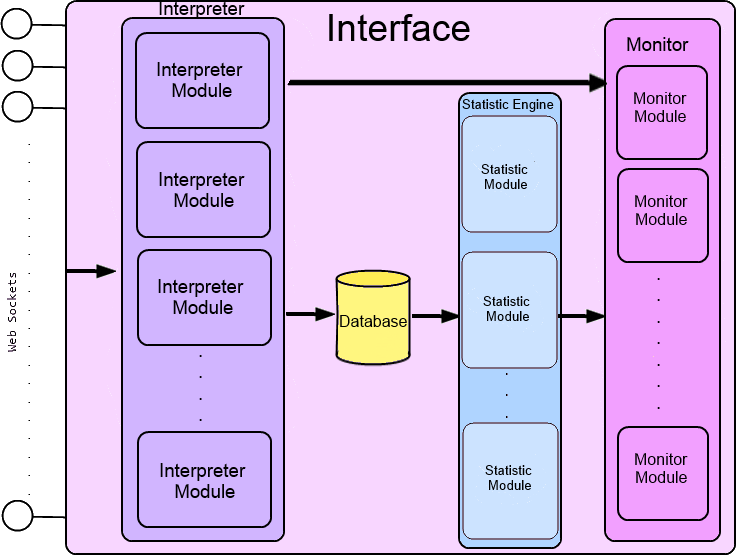
\includegraphics[scale=0.6]{Interface.png}
\caption{The Architecture}
\label{threadsVsSync}
\end{figure}

\subsubsection{Interpreter}
Containing several interpreter modules, the interpreter serves as the brain of the interface receiving the data (initially received through the sockets) and then begins digesting and translating it into actual info. It then sends it to the monitor (to display the data received) and the database manager (to save the data).

\begin{figure}[h!]
\centering
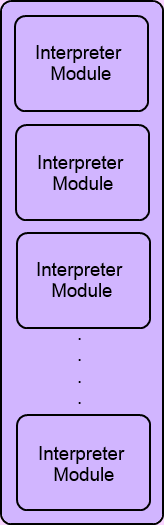
\includegraphics[height=60mm]{Interpreter.png}
\caption{The Interpreter}
\label{threadsVsSync}
\end{figure}

\subsubsection{Database engine}
The database engine saves the users and their data; this data, or history, is collected from previous sessions the trainee took.

\subsubsection{Statistics engine}
Containing several statistics modules, this engine generates the analysis (this analysis depends on the current data received + the history of the trainee) and sends it to the monitor.

\begin{figure}[h!]
\centering
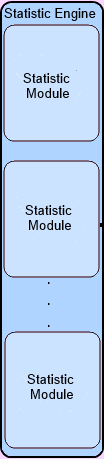
\includegraphics[height=60mm]{Statistics.png}
\caption{The Statistics Engine}
\label{threadsVsSync}
\end{figure}

\newpage

\subsubsection{Monitor}
The monitor is the front end component of the interface that displays all the info (including live data and statistics-related data). It contains several monitoring modules together make up the monitor.

\begin{figure}[h!]
\centering
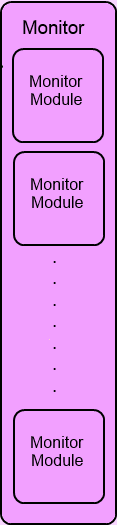
\includegraphics[height=55mm]{Monitor.png}
\caption{The Monitoring System}
\label{threadsVsSync}
\end{figure}

\subsection{Hand shaking}
This is the process where each plugin reserves a web socket to start the data stream with the interface. This begins when the plugin sends a request to the interface via a socket, then the interface reserves the socket for the plugin and sends an OK signal. Once the OK signal is received, the plugin can start the data stream at any time.

\subsection{Data stream}
The data stream contains the type of the data sent (on-session or off-session), a timestamp and the actual data. Depending on the type of the sensor sending the data, the actual data will differ. These data stream elements will be received by the front-end of the monitor, which in turn sends it to the back-end layer to interpret. The back-end layer then parses the data, saves it in the database and sends it back to the front-end layer (this time only the actual data is sent). The front-end layer displays the data according to its type.

\subsection{The Implementation}
The application is coded using Django (a Python based framework), SQLite, HTML, CSS3, Jquery and Javascript. Python and SQLite are used to implement the back-end layer, while HTML, CSS3, JavaScript, jQuery and Ajax are for the front-end layer.

\subsubsection{Back-end layer}
This layer is the one responsible for the work done in the engine of the application. It does the part of the work invisible to the user and serves indirectly as a support for the front-end layer, usually by being closer to the required resource or database, or having the capability to communicate with the required resource or database

\newpage

\paragraph{Python}
Conceived in the late 1980s by Guido van Rossum, Python is a general-purpose, high-level programming language with a syntax that allows developers to express concepts in fewer lines of code than would be possible in languages such as C, C++, Java. It supports multiple programming paradigms such as imperative, object-oriented and functional programming paradigms. It also features a dynamic type system and automatic memory management and has a large and comprehensive standard library. Python is often used as a scripting language, but is also used in a wide range of non-scripting contexts with its interpreters available for many operating systems.

Python is used to implement the logic of the monitor. This logic serves as the engine of the monitor that handles all the data received, generating the statistics and communication between the database and the front-end layer.

\paragraph{SQLite}
Designed in the spring of 2000 by D. Richard Hipp, SQLite is a relational database management system contained in a C programming library. Unlike client–server database management systems, the SQLite engine has no standalone processes with which the application program communicates. Instead, the SQLite library is linked in and thus becomes an integral part of the application program. It is a popular choice as embedded database for local/client storage in application software such as web browsers. It is the most widely deployed database engine, as it is used today by several widespread browsers, operating systems, and embedded systems, among others.

SQLite is used to store all the data that would be needed for future use. This data include the practitioners' basic info (usernames and passwords), sessions' info (start time, end time, duration and off-round measurements), rounds' info (start time, end time, duration and on-round measurements + data) and statistics.

\subsubsection{Front-end layer}
This layer does the part of the work visible to the users. It is the one that the users interact with directly.

\paragraph{HTML}
HTML stands for HyperText Markup Language. It is the main markup language for creating web pages and other information that can be displayed in a web browser. It is written in the form of HTML elements consisting of tags enclosed in angle brackets (like <html>), within the web page content. In between these tags, text, tags, comments and other types of text-based content can be added.

HTML is used to layout the monitor's user interface UI.

\newpage

\paragraph{CSS3}
CSS stands for Cascading Style Sheets. It is a style sheet language used for describing the presentation semantics (the look and formatting) of a document written in a markup language. Its most common application is to style web pages written in HTML and XHTML, but the language can also be applied to any kind of XML document, including plain XML, SVG and XUL. It is designed primarily to enable the separation of document content (written in HTML or a similar markup language) from document presentation, including elements such as the layout, colors, and fonts. This separation can improve content accessibility, provide more flexibility and control in the specification of presentation characteristics, enable multiple pages to share formatting, and reduce complexity and repetition in the structural content.

CSS3 is used to design the layout created by HTML.

\paragraph{JavaScript}
JavaScript is an interpreted computer programming language originally implemented as part of web browsers so that client-side scripts could interact with the user, control the browser, communicate asynchronously, and alter the document content that was displayed. Now though it has many uses involving popular game development and the creation of applications.

\paragraph{jQuery}
Released in January 2006 at BarCamp NYC by John ResigjQuery, jQuery is a multi-browser JavaScript library designed to simplify the client-side scripting of HTML. It is currently developed by a team of developers led by Dave Methvin. Used by over 65\% of the 10,000 most visited websites, jQuery is the most popular JavaScript library in use today.

JavaScript and jQuery are used to code the logic part needed in the front-end layer. This logic includes the starting and stopping of the rounds and sessions, the stopwatch/timer and displaying the data received from the back-end layer (after the data is parsed).

\paragraph{Ajax}
Ajax is a group of interrelated web development techniques used on the client-side to create asynchronous web applications. With Ajax, web applications can send data to, and retrieve data from, a server asynchronously (in the background) without interfering with the display and behavior of the existing page. Data can be retrieved using the XMLHttpRequest object. The use of XML is not required (JSON is often used instead), and the requests do not need to be asynchronous.

Ajax is used to allow the data received from the sensors to be sent through the front-end layer to the back-end layer in the background (in a "live" style). It is also used to send data from the back-end layer to the front-end layer and displaying it without interfering with the ongoing processes.

\subsection{The features}
The application consists of three main features, live session monitoring, statistics and a small social part.

\newpage

\subsubsection{Live session monitoring}
In this feature, the user creates a session (with a number of rounds, round duration and break duration) and then connects the sensor(s) needed and can do off-session measurements. Then the user starts the session and records the actions done.

One of the biggest challenges faced during the implementation of this feature was that the rounds should be saved to the database very quickly that the user won't notice that their is something happening in the background of the application. A proposed solution was that the round is saved at the end of it, this caused a small lag in the timer (this was very noticeable in sessions that had a short break between the rounds). The solution implemented was creating and saving the rounds objects to the database while creating the session and then when something is needed to be updated in the round's data, it is saved during the round, therefore minimizing the number of queries executed during the session.

\paragraph*{Insert Live session figure here.}

\subsubsection{Statistics}

This feature serves to show the practitioners their progress over time. They can see their best-done moves, frequent-done moves, moves they need to practice on, rate of their moves with respect to the round's duration and other session-related info.

\paragraph*{Insert statistics figure here.}

\subsubsection{Social}

In this feature, the practitioners can check other practitioners' level, progress and session data. The main reason behind this is to give the application a bit of gaming taste.

\paragraph*{Insert social figure here.}

\end{document}

%%% Local Variables: 
%%% mode: latex
%%% TeX-master: t
%%% End: 
